%%%%%%%%%%%%%%%%%%%%%%%%%%%%%%%%%%%%%%%%%
% University/School Laboratory Report
% LaTeX Template
% Version 3.1 (25/3/14)
%
% This template has been downloaded from:
% http://www.LaTeXTemplates.com
%
% Original author:
% Linux and Unix Users Group at Virginia Tech Wiki 
% (https://vtluug.org/wiki/Example_LaTeX_chem_lab_report)
%
% License:
% CC BY-NC-SA 3.0 (http://creativecommons.org/licenses/by-nc-sa/3.0/)
%
%%%%%%%%%%%%%%%%%%%%%%%%%%%%%%%%%%%%%%%%%

\documentclass{article}
\usepackage[utf8]{inputenc}
\usepackage{appendix}
\usepackage[T1]{fontenc}
\usepackage{siunitx} % Provides the \SI{}{} and \si{} command for typesetting SI units
\usepackage{graphicx} % Required for the inclusion of images
\usepackage{natbib} % Required to change bibliography style to APA
\usepackage{amsmath} % Required for some math elements 
\usepackage{caption}
\usepackage{tikz}

\usetikzlibrary{arrows,automata, positioning}

\usepackage{import}

\setlength\parindent{0pt} % Removes all indentation from paragraphs

\title{Prova Finale di Reti Logiche} % Title
\author{Vincenzo Greco} % Author name
\date{May 16th, 2021}

\begin{document}
\maketitle % Insert the title, author and date
\begin{center}
\begin{tabular}{l r}
Matricola: & 916368\\ % Partner names
Codice Persona: & 10683567\\
Docente: & Salice Fabio	 % Instructor/supervisor
\end{tabular}
\end{center}

\section{Requisiti del Progetto}

Il progetto richiesto consiste nell'implementazione in VHDL dell metodo di \textbf{
equalizzazione dell’istogramma di una immagine}.\\
Data un'immagine salvata in memoria viene chiesto al componente di:
\begin{enumerate}
\item Accedere ad una memoria RAM per recuperare il numero di righe e colonne di pixel di cui e' composta l'immagine
\item Iterare nella memoria per trovare minimo e massimo dei valori dei pixel
\item Trovare il livello di shift da applicare ad ogni pixel dell'immagine
\item Calcolare il nuovo valore dei pixel e salvarli in memoria
\end{enumerate}

La massima grandezza della matrice dell'immagine e' 128 x 128 come da specifica. Nel caso fosse letto un valore maggiore di righe o colonne questo verra' salvato come 128. Nel caso di presenza di valori oltre l' indice di righe x colonne, questi verranno, nel caso fossero raggiunti, sovrascritti dai pixel pixel equalizzati.\\
Inoltre, l'implementazione deve essere in grado di gestire un segnale di Reset. Per l'implementazione si è scelto di supporre il Reset asincrono rispetto al segnale di clock. L'implementazione deve essere poi sintetizzata con target a FPGA xc7a200tfbg484-1.

\newpage
\noindent

%----------------------------------------------------------------------------------------
%	SECTION 2
%----------------------------------------------------------------------------------------

\section{Implementazione}

\subsection{Descrizione ad Alto Livello}
\label{alto_livello}

Da un'ottica di alto livello, l'implementazione esegue i seguenti passi:

\begin{enumerate}
\item Carica il numero di righe e colonne della matrice dei pixel dalla RAM
\item Esegue la ricerca di massimi e minimi:
\item Calcola il valore dello shift.
\item Per ogni pixel in memoria calcola il valore del pixel equalizzato e lo salva in RAM
\item Ad operazione conclusa il componente comunica il suo stato di done fin quando non verra' indicato che la prossima immagine e' disponibile all' equalizzazione
\end{enumerate}

\subsection{Macchina a Stati Finiti}
\label{FSM}

La FSM è stata realizzata con specifica behavioural mediante due processi: \texttt{STATE} e \texttt{DELTA\_LAMBDA}.

Il processo \texttt{STATE} è il processo che si occupa di cambiare lo stato sul fronte di salita del clock e di portare la macchina nello stato di reset se questo fosse rilevato.
Il processo \texttt{DELTA\_LAMBDA} è invece il processo combinatorio che calcola le uscite e lo stato validi per il prossimo fronte di salita del clock.

Gli stati della FSM sono:

\begin{itemize}
\item \texttt{RST}: Stato in cui la macchina si prepara che il segnale \texttt{i\_start} venga portato alto per poter iniziare l'esecuzione. Queseto stato si occupa anche di portare i segnali interni in uno stato consistente per l'esecuzione.
\item \texttt{SAVE\_COLUMN}: Stato in cui si legge dalla RAM l'indirizzo 1 della memoria che corrisponde al numero di colonne che compongono l'immagine. Il valore salvato sara' il minimo fra quello fronito da \texttt{i\_data} e 128. Nel caso il valore fosse 0 il processo porta l'\texttt{o\_done} alto.
\item \texttt{SAVE\_ROW}: Stato in cui si legge dalla RAM l'indirizzo 0 della memoria che corrisponde al numero di righe che compongono l'immagine. Il valore salvato sara' il minimo fra quello fronito da \texttt{i\_data} e 128. Nel caso il valore fosse 0 il processo porta l'\texttt{o\_done} alto.
\item \texttt{SAVE\_PIXEL}: Stato in cui si legge il valore del pixel e li confrontano con massimi e minimi.
\item \texttt{LOOP\_SAVE}: Stato in cui decide se siano stati letti tutti i valori della matrice di pixel
\item \texttt{CALC\_SHIFT }: Stato in cui si calcola lo shift
\item \texttt{EQUALIZE\_PIXEL}: Stato in cui si calcola il valore aggiornato di un pixel al seguito della equalizzazione
\item \texttt{SAVE\_PIXEL\_EQUALIZED}: Stato in cui viene salvato il pixel in RAM
\item \texttt{LOOP\_SAVE\_EQUALIZED }: Stato in cui si decide se siano stati equalizzati tutti i pixel della matrice
\item \texttt{DONE}: Stato in cui si aspetta che \texttt{i\_start} venga portato basso e riportandosi allo stato di \texttt{RST}.
\end{itemize}

Nella figura a seguito è riportato il disegno dell'automa.


\begin{center}
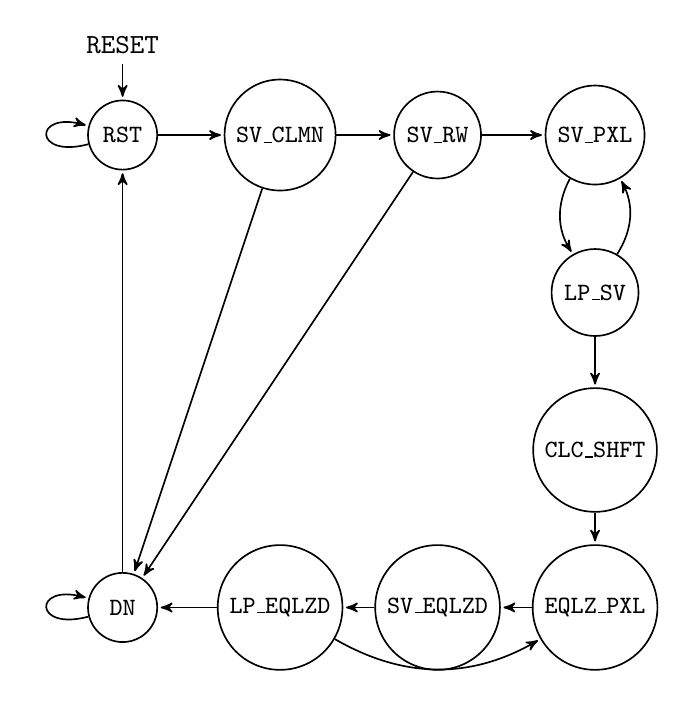
\begin{tikzpicture}[->,>=stealth',shorten >=1pt,auto,node distance=2cm,
                    semithick, initial where=above, initial text={\texttt{RESET}}]

  \tikzstyle{every state} = [font=\small]
  \node[initial,state] (A)                    {\texttt{RST}};
  \node[state]         (B) [right of=A] 	  {\texttt{SV\_CLMN}};
  \node[state]         (C) [right of=B] 	  {\texttt{SV\_RW}};
  \node[state]         (D) [right of=C] 	  {\texttt{SV\_PXL}};
  \node[state]         (E) [below of=D]       {\texttt{LP\_SV}};
  \node[state]         (F) [below of=E]       {\texttt{CLC\_SHFT}};
  \node[state]         (G) [below of=F]       {\texttt{EQLZ\_PXL}};
  \node[state]         (H) [left of=G]       {\texttt{SV\_EQLZD}};
  \node[state]         (I) [left of=H]       {\texttt{LP\_EQLZD}};
  \node[state]         (J) [left of=I]       {\texttt{DN}};

  \path (A) edge              node {} (B)
 	    (A) edge  [loop left] node {} (A)
        (B) edge              node {} (C)
        (B) edge              node {} (J)
        (C) edge              node {} (D)
        (C) edge              node {} (J)
        (D) edge 	[bend right]		  node {} (E)
        (E) edge 			  node {} (F)
        (E) edge 	[bend right]		  node {} (D)
        (F) edge 			  node {} (G)
        (G) edge 			  node {} (H)
        (H) edge			  node {} (I)
        (I) edge			  node {} (J)
        (I) edge	[bend right]		  node {} (G)
        (J) edge			  node{} (A)
        (J) edge	[loop left]		  node {} (J);
\end{tikzpicture}
\end{center}

\newpage

\section{Test Benches}
\label{test}

I test sono stati effettutati allo scopo di trovari eventuali criticita' del componente

\begin{itemize}
\item Segnale di \texttt{RESET} asincrono rispetto al clock
\item Valore di righe e/o colonne a 0 controllando che quindi nessun valore in RAM venga modificato
\item Matrice di pixel 1 x 1 e 128 x 128 per testare le dimensioni limite dell'immagine
\item Altri test bench vari generati casualmente, mantenendo la validità della specifica
\end{itemize}

Per tutti i test riportati e i test successivi è stata effettuata la simulazione behavioural e successivamente la simulazione functional e timing post-synthesis, tutte con successo.\\

\section{Risultati Sperimentali}
\label{risultati}

\subsection{Report di Sintesi}

Dal punto di vista dell'area la sintesi riporta il seguente utilizzo dei componenti:
\begin{itemize}
\item LUT: 173 (0.13\% del totale)
\item FF: 112 (0.04\% del totale)
\end{itemize}

\subsection{Risultato dei Test Bench}

Lavorando sul testing si è anche provato a variare il periodo di clock, confermando che, non solo l'implementazione mantiene il suo funzionamento anche a \SI{1}{\ns} nella simulazione Behavioural e \SI{2}{\ns} nella simulazione Functional Post-Synthesis. Test inferiori a 1ns non sono stati effettuati.\\

\section{Conclusioni}

Avendo passato la totalita' dei test sia scritti manualmente, che generati, che ricevuti attraverso beep o altri canali di comunicazione, posso affermare con una certa confidenza che l'implementazione rispetti tutte le specifiche indicate.
\end{document}
